% Compact PGFPlots panel for sampled gross144 BSC correction-class derivative.
% Requires \usepackage{pgfplots} and \pgfplotsset{compat=1.18}.
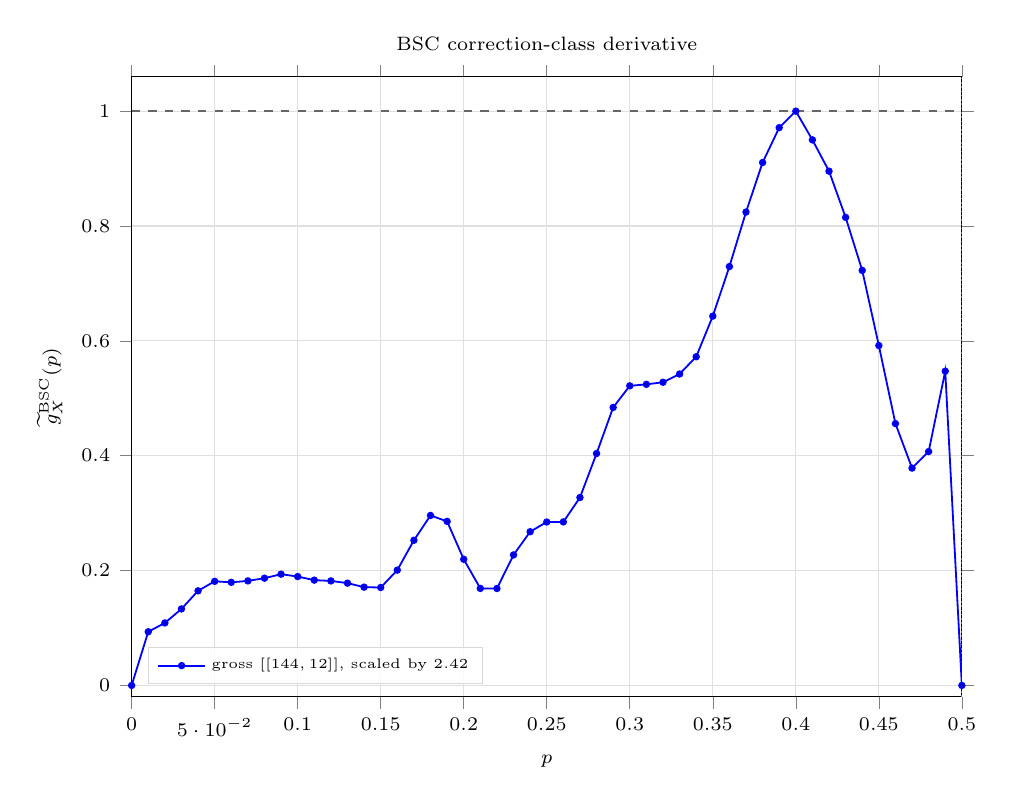
\begin{tikzpicture}
\begin{axis}[
  name=scaledBSCGEXITGross144Axis,
  width=\linewidth,
  height=0.78\linewidth,
  title={BSC correction-class derivative},
  title style={font=\scriptsize},
  xlabel={$p$},
  ylabel={$\widetilde g_X^{\rm BSC}(p)$},
  xmin=0, xmax=0.5,
  ymin=-0.02, ymax=1.06,
  grid=both,
  major grid style={black!12},
  minor grid style={black!6},
  tick align=outside,
  tick label style={font=\scriptsize},
  label style={font=\scriptsize},
  legend cell align={left},
  legend style={draw=black!15, fill=white, fill opacity=0.82, text opacity=1, at={(0.02,0.02)}, anchor=south west, font=\tiny},
]
\addplot[black!60, densely dotted, line width=0.55pt, forget plot] coordinates {(0.5,-0.02) (0.5,1.06)};
\addplot[black!60, dashed, line width=0.55pt, forget plot] coordinates {(0,1) (0.5,1)};
\addplot+[color=blue, mark=*, mark size=1.0pt, line width=0.65pt]
coordinates {(0,0) (0.01,0.0934577977967) (0.02,0.10879035072) (0.03,0.133226565242) (0.04,0.164746069912) (0.05,0.181282468256) (0.06,0.17950239662) (0.07,0.182003820468) (0.08,0.18672118812) (0.09,0.193717734772) (0.1,0.189528570276) (0.11,0.183342515398) (0.12,0.182000550606) (0.13,0.178110176292) (0.14,0.171120571227) (0.15,0.170494090153) (0.16,0.200794151465) (0.17,0.25279041604) (0.18,0.296018787996) (0.19,0.285623586337) (0.2,0.219647654278) (0.21,0.168890134145) (0.22,0.168784966026) (0.23,0.227276197179) (0.24,0.267628762263) (0.25,0.284594986822) (0.26,0.284738312593) (0.27,0.327237355352) (0.28,0.403854594702) (0.29,0.484085967126) (0.3,0.521694742327) (0.31,0.524285965862) (0.32,0.527940677736) (0.33,0.542292935436) (0.34,0.572356214568) (0.35,0.643097793893) (0.36,0.729405534168) (0.37,0.824315509669) (0.38,0.91057960113) (0.39,0.971337695363) (0.4,1) (0.41,0.949991043222) (0.42,0.895525134013) (0.43,0.815060611111) (0.44,0.722661316831) (0.45,0.591904996846) (0.46,0.455973354635) (0.47,0.378474689224) (0.48,0.407245775201) (0.49,0.547242136341) (0.5,0)};
\addlegendentry{gross $[[144,12]]$, scaled by $2.42$}
\end{axis}
\end{tikzpicture}
